
%(BEGIN_QUESTION)
% Copyright 2014, Tony R. Kuphaldt, released under the Creative Commons Attribution License (v 1.0)
% This means you may do almost anything with this work of mine, so long as you give me proper credit

Bruk ``impedanstrekanten'' for å beregne impedansen i denne seriekombinasjonen av resistans ($R$) og induktiv reaktans ($X$):

$$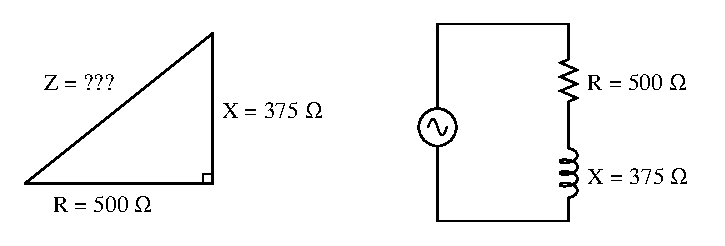
\includegraphics[width=15.5cm]{i01030x01.eps}$$

Forklar hvilke ligninger du bruker for å beregne $Z$.

\underbar{file i01030}
%(END_QUESTION)





%(BEGIN_ANSWER)

$Z$ = 625 $\Omega$, beregnet med Pythagoras' teorem.

%(END_ANSWER)





%(BEGIN_NOTES)

Be studentene vise formen på Pythagoras' teorem selv, i stedet for at du gir den direkte.

%INDEX% Electronics review: AC reactance and impedance

%(END_NOTES)

